\begin{frame}{Solução Proposta: Processo de Desenvolvimento}
\begin{itemize}
	\item Processo de Desenvolvimento Adotado: \alert{Processo Unificado Ágil}
	\begin{itemize}
		\item Fases e disciplinas
		\item Concepção, elaboração, construção e transição
	\end{itemize}
	\ \ \newline
	\item Aplicação a ser desenvolvida não é considerada de grande porte
	\ \ \newline
	\item Papéis:
	\begin{itemize}
		\item Desenvolvedor e testador: Pedro Augusto
		\item Cliente: Profa. Maria Betânia
		\item Solicitante do software e Gerente do Projeto: Profa. Elloá
	\end{itemize}
\end{itemize}
\end{frame}

\begin{frame}{Solução Proposta}
\begin{block}{Elicitação de Requisitos}
\begin{itemize}
	\item Identificação dos requisitos funcionais e não funcionais
	\item Identificação de quatro módulos principais:
	\begin{enumerate}
		\item Módulo Gerencia Conta de Usuário
		\item Módulo Usuário
		\item Módulo Consulta Medições
		\item Módulo Gerencia Medições
	\end{enumerate}
\end{itemize}
\end{block}

\end{frame}

\begin{frame}{Solução Proposta: Diagramas de Caso de Uso}
\begin{figure}[h!]
\centering
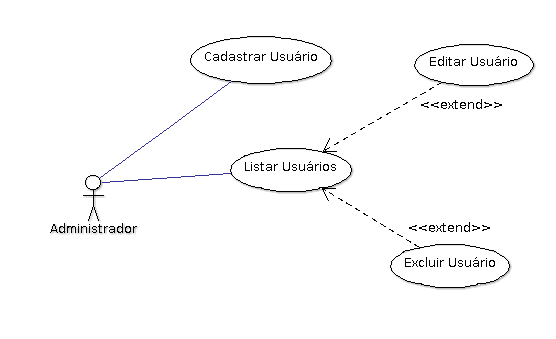
\includegraphics[width=0.8\linewidth]{./img/uc001}
\end{figure}
\end{frame}

\begin{frame}{Solução Proposta: Diagramas de Caso de Uso}
\begin{figure}[h!]
\centering
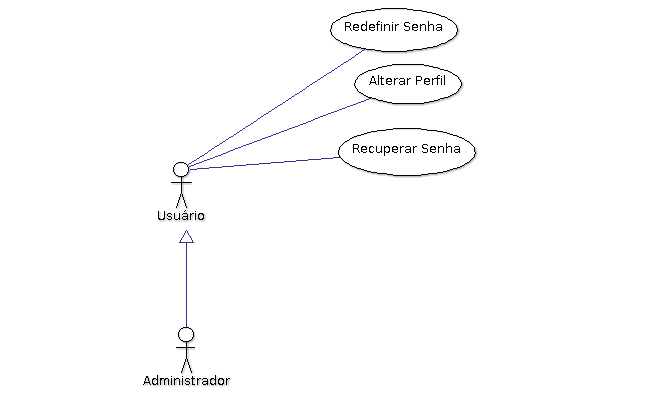
\includegraphics[width=0.7\linewidth]{./img/uc002}
\end{figure}
\end{frame}

\begin{frame}{Solução Proposta: Diagramas de Caso de Uso}
\begin{figure}[h!]
\centering
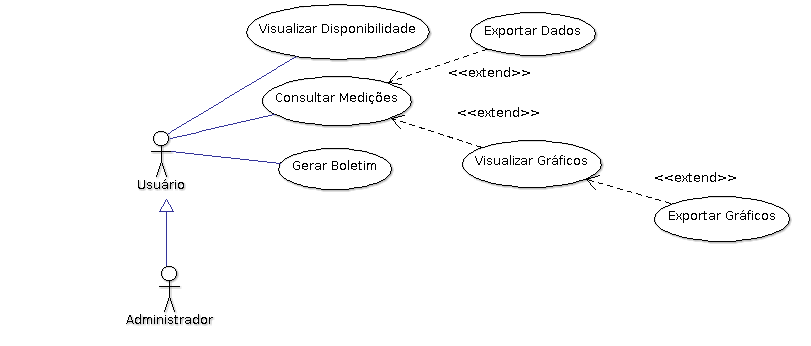
\includegraphics[width=1\linewidth]{./img/uc003}
\end{figure}
\end{frame}

\begin{frame}{Solução Proposta: Diagramas de Caso de Uso}
\begin{figure}[h!]
\centering
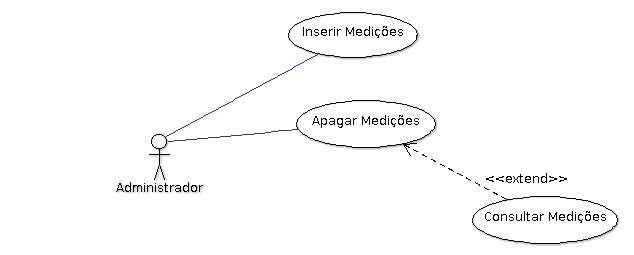
\includegraphics[width=1\linewidth]{./img/uc004}
\end{figure}
\end{frame}


\begin{frame}{Solução Proposta}
\begin{block}{Elaboração de Modelos}
\begin{itemize}
	\item Identificação das principais abstrações efetuadas e da associação entre elas
	\item Modelo Conceitual
	\item Modelo Entidade-Relacionamento
\end{itemize}
\end{block}
\end{frame}

\begin{frame}{Solução Proposta: Modelo Conceitual}
	\begin{figure}[h!]
	\centering
	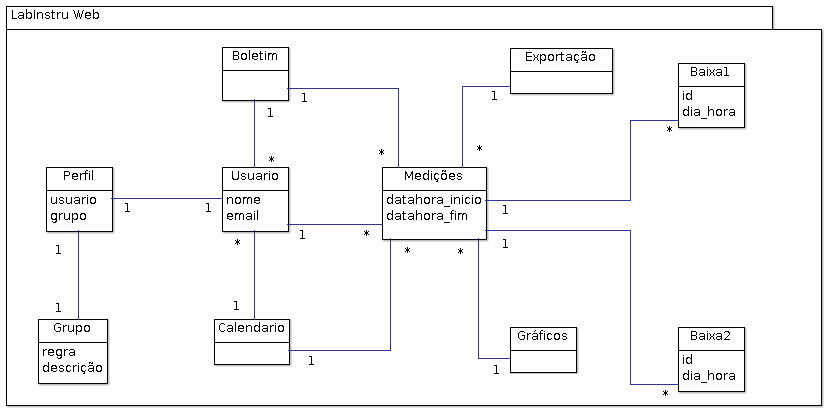
\includegraphics[width=0.8\linewidth]{./img/ModeloConceitual}
	\end{figure}
\end{frame}

\begin{frame}{Solução Proposta: Modelo Entidade-Relacionamento}
	\begin{figure}[h!]
	\centering
	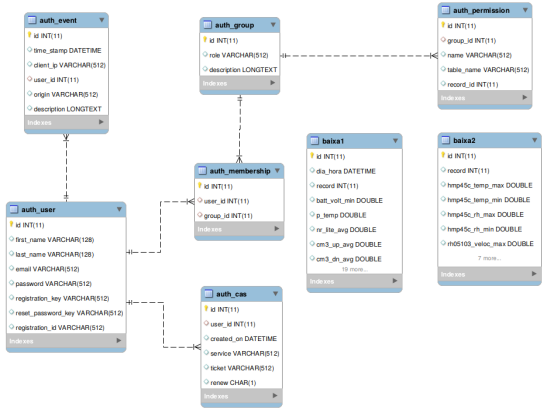
\includegraphics[width=0.6\linewidth]{./img/mer}
	\end{figure}
\end{frame}

\begin{frame}{Solução Proposta}
\begin{block}{Prototipação das Telas do Usuário}
\begin{itemize}
	\item Elaboração de protótipos da interface com o usuário
	\item Representação limitada da solução, mas capaz de explorar a sua conveniência
	\item Utilização do Balsamiq Mockups
\end{itemize}
\end{block}
\end{frame}

\begin{frame}{Solução Proposta: Prototipação}
\begin{figure}[h!]
\centering
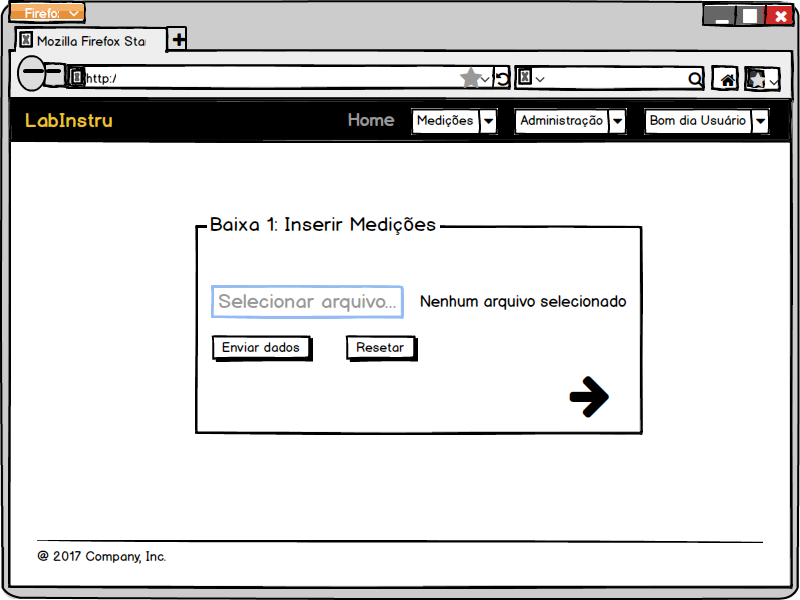
\includegraphics[width=0.6\linewidth]{./img/tela053}
\caption{Protótipo cadastra medições} \label{fig:uc001}
\end{figure}
\end{frame}

\begin{frame}{Solução Proposta: Prototipação}
\begin{figure}[h!]
\centering
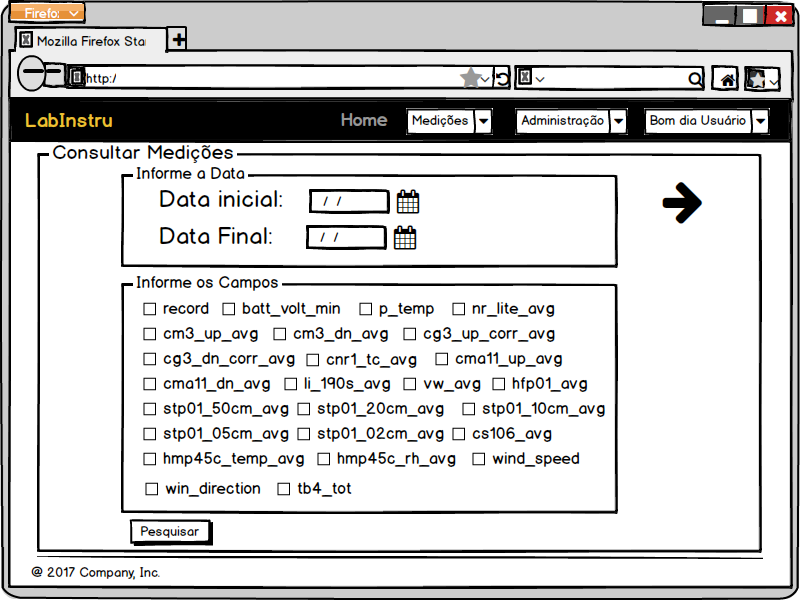
\includegraphics[width=0.6\linewidth]{./img/tela058}
\caption{Protótipo consulta medições} \label{fig:uc001}
\end{figure}
\end{frame}



\begin{frame}{Solução Proposta}
	\begin{block}{Implementação}
		\begin{itemize}
			\item \alert{LabInstru Web}: plataforma web proposta para atender às necessidades identificadas no LabInstru
			\ \ \newline
			\item \emph{Framework} utilizado: Web2py
				\begin{itemize}
					\item Programável e escrito em Python
					\item Utiliza o MVC como padrão de projeto
				\end{itemize}
			\ \ \newline
			\item Melhorias na interface com o usuário:
			\begin{itemize}
				\item \emph{Framework} Bootstrap
				\item Biblioteca JQuery
			\end{itemize}
			\ \ \newline
			\item Sistema gerenciador de Banco de Dados: MySQL
		\end{itemize}
	\end{block}
\end{frame}

\begin{frame}{Solução Proposta: Funcionalidades Implementadas}
\begin{figure}[h!]
\centering
\frame{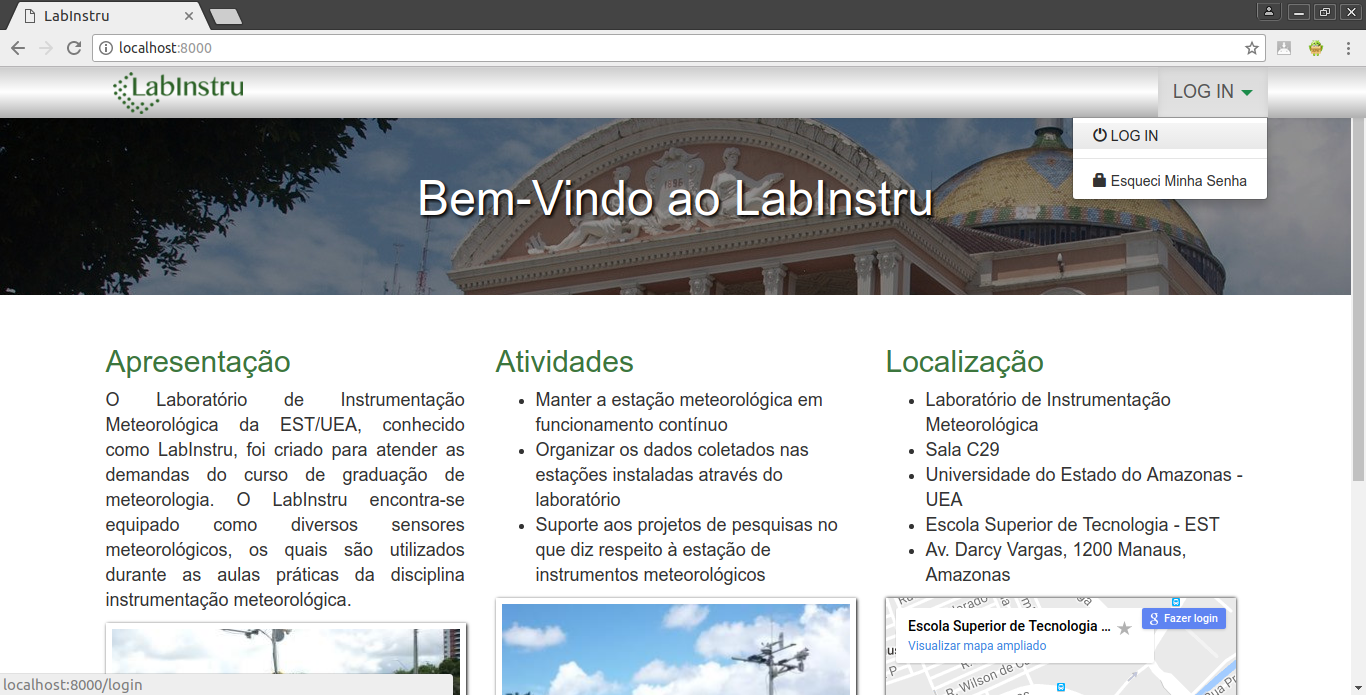
\includegraphics[width=0.7\linewidth]{./img/ap1}}
\caption{Página inicial da aplicação.}
\end{figure}
\end{frame}

\begin{frame}{Solução Proposta: Funcionalidades Implementadas}
\begin{figure}[h!]
\centering
\frame{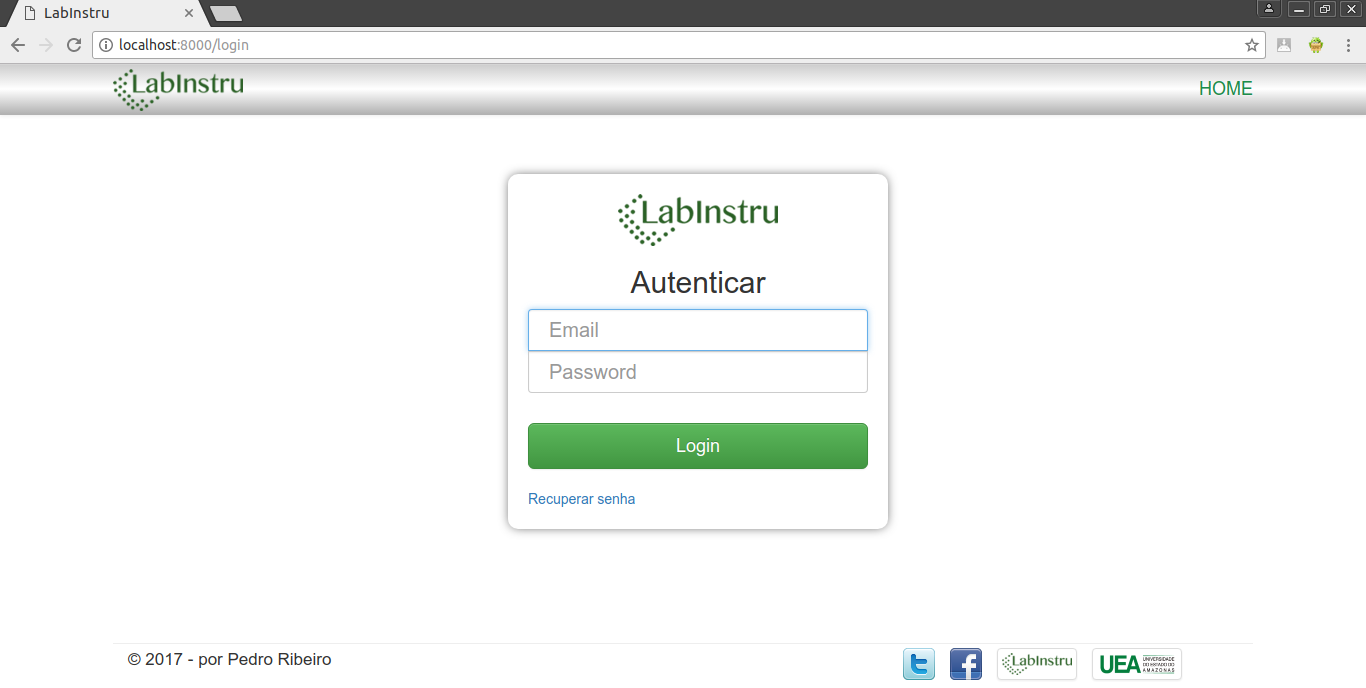
\includegraphics[width=0.7\linewidth]{./img/ap10}}
\caption{Autenticação de usuários.}
\end{figure}
\end{frame}

\begin{frame}{Solução Proposta: Funcionalidades Implementadas}
\begin{figure}[h!]
\centering
\frame{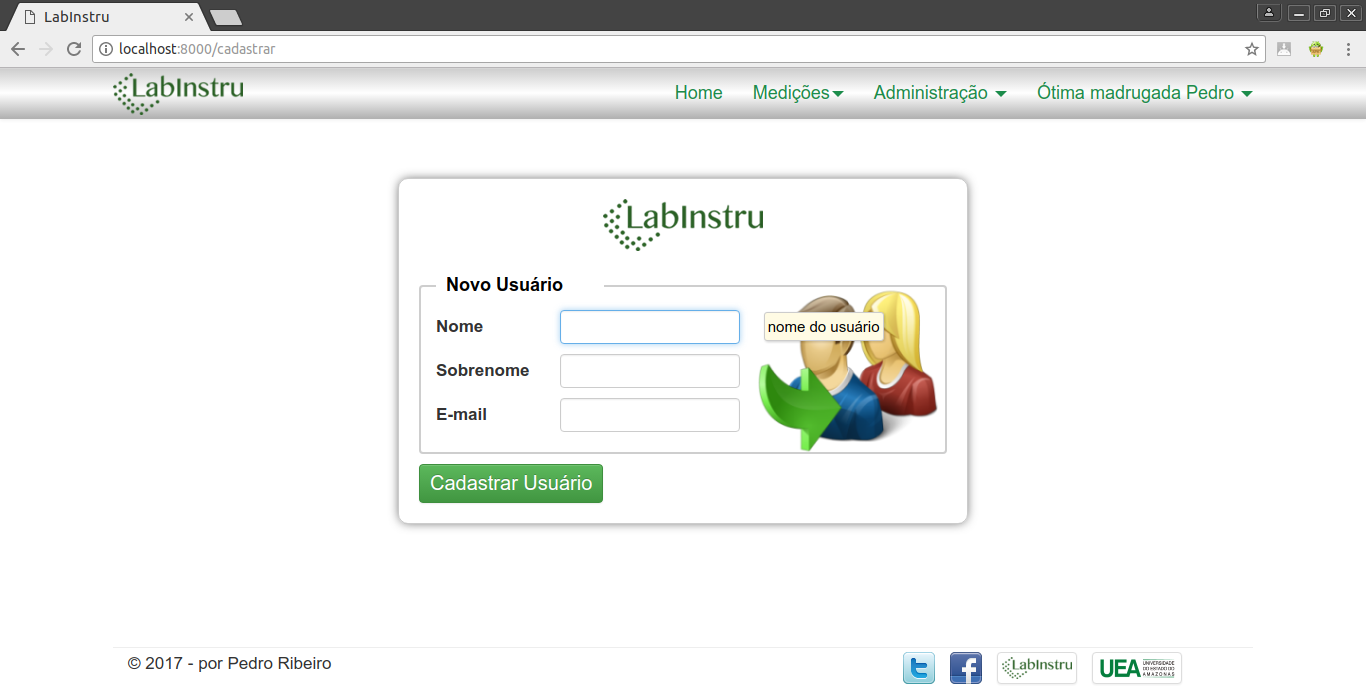
\includegraphics[width=0.7\linewidth]{./img/ap4}}
\caption{Cadastro de usuários.}
\end{figure}
\end{frame}

\begin{frame}{Solução Proposta: Funcionalidades Implementadas}
\begin{figure}[h!]
\centering
\frame{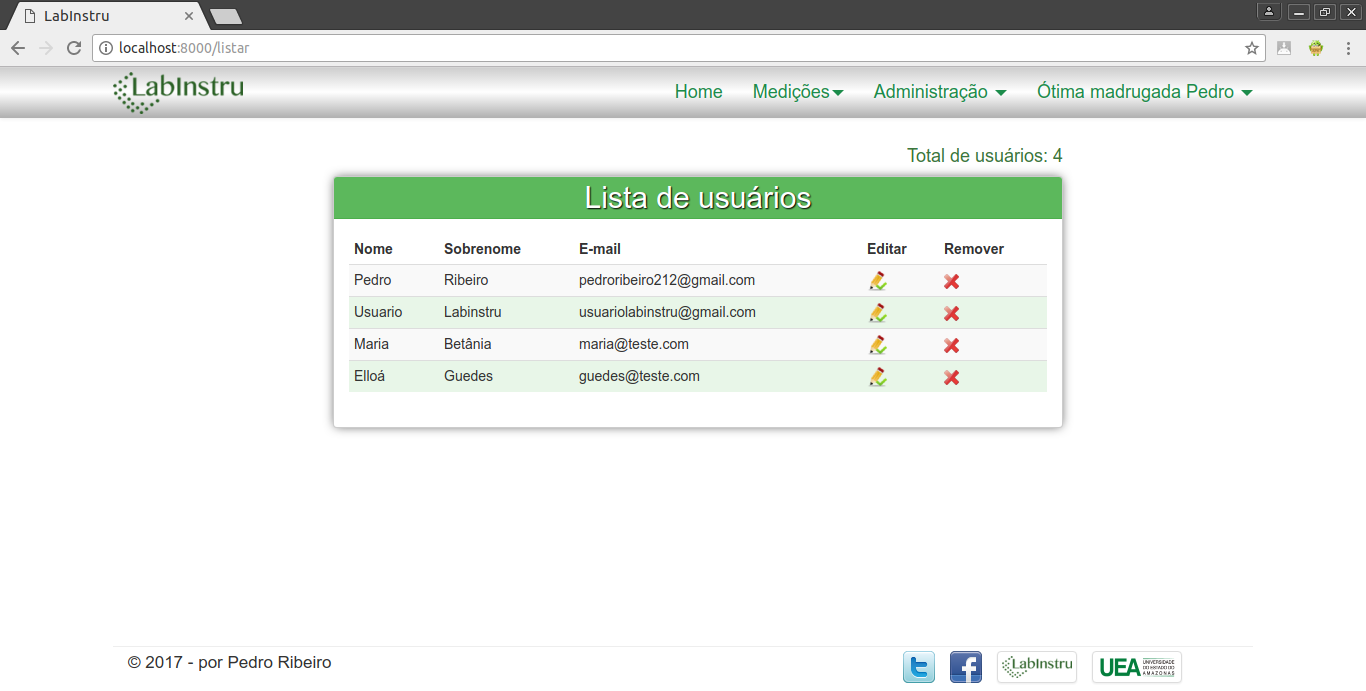
\includegraphics[width=0.7\linewidth]{./img/ap14}}
\caption{Listagem de usuários.}
\end{figure}
\end{frame}


\begin{frame}{Solução Proposta: Funcionalidades Implementadas}
\begin{figure}[h!]
\centering
\frame{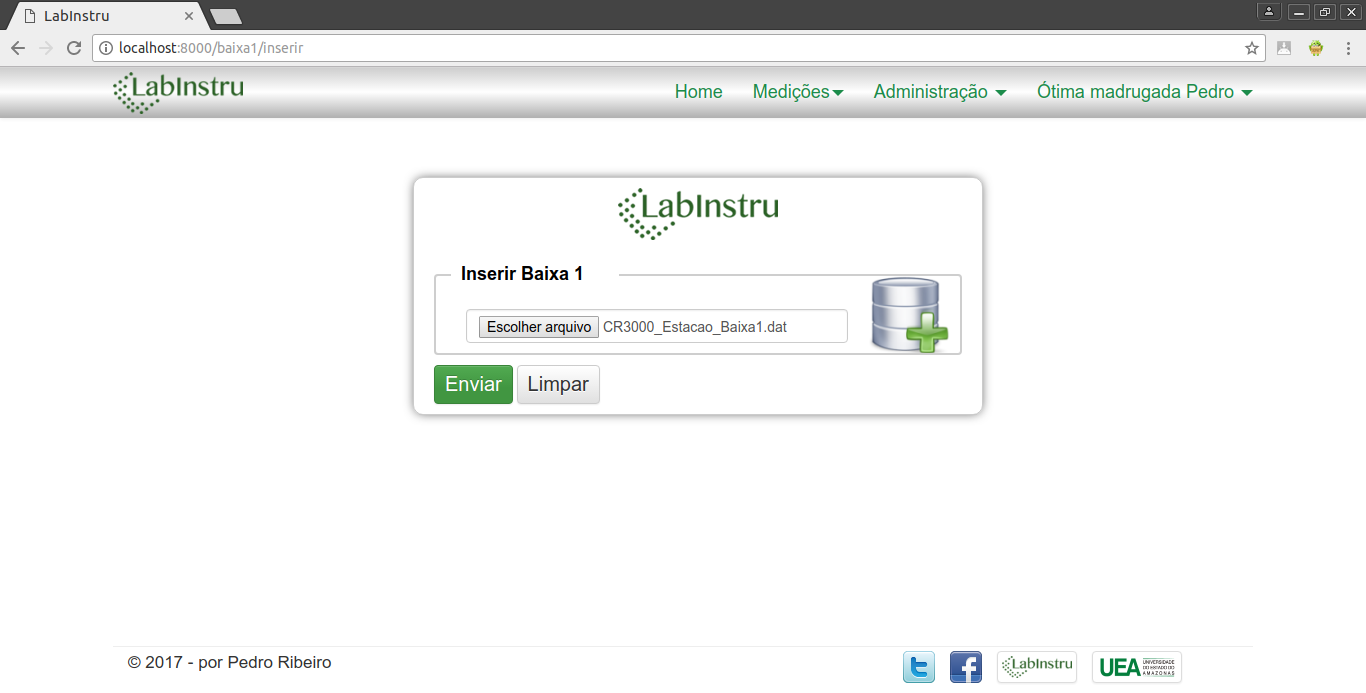
\includegraphics[width=0.7\linewidth]{./img/ap12}}
\caption{Cadastro de Medições.}
\end{figure}
\end{frame}

\begin{frame}{Solução Proposta: Funcionalidades Implementadas}
\begin{figure}[h!]
\centering
\frame{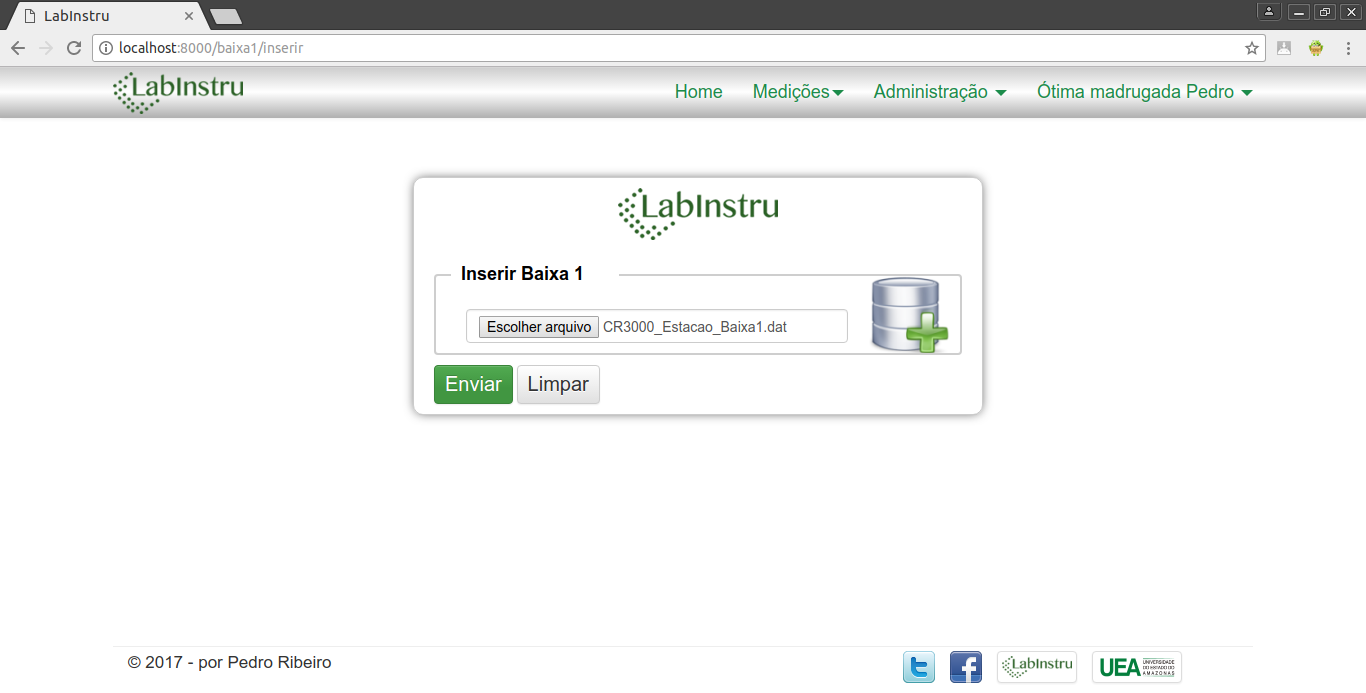
\includegraphics[width=0.7\linewidth]{./img/ap12}}
\caption{Cadastro de Medições.}
\end{figure}
\end{frame}

\begin{frame}{Solução Proposta: Funcionalidades Implementadas}
\begin{figure}[h!]
\centering
\frame{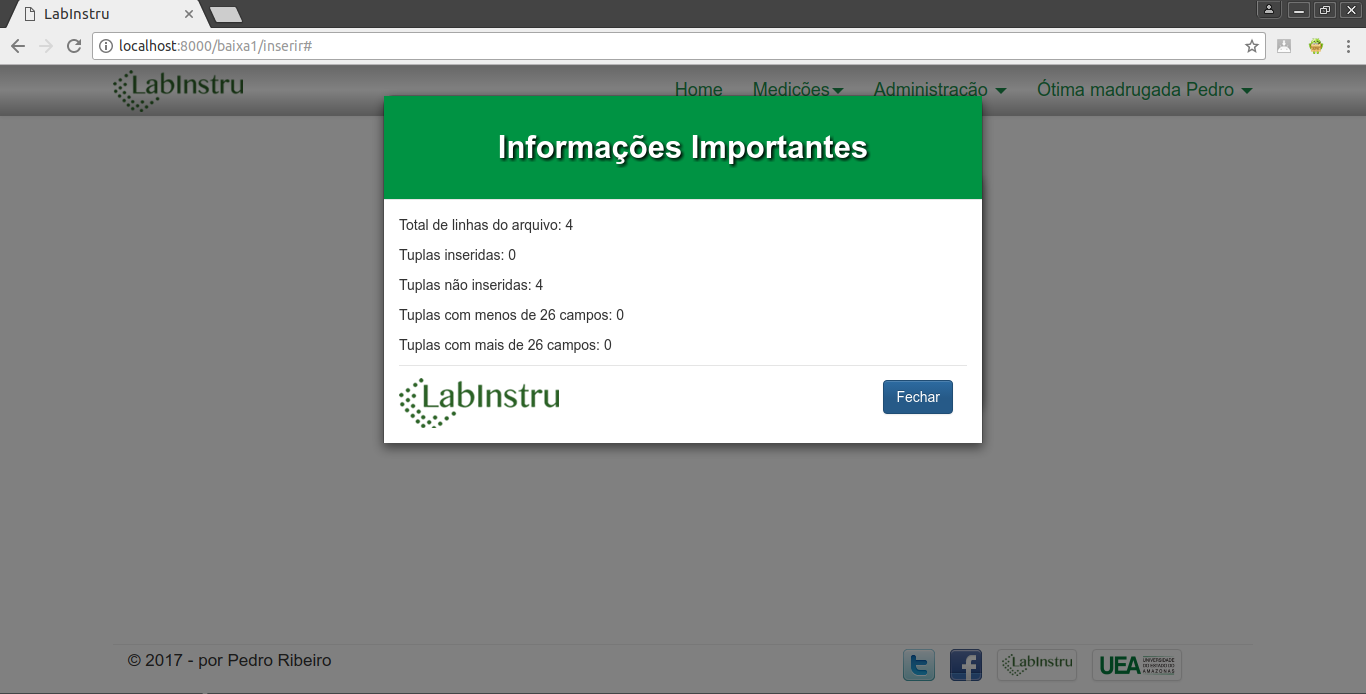
\includegraphics[width=0.7\linewidth]{./img/ap13}}
\caption{Log resultante do cadastro de Medições.}
\end{figure}
\end{frame}

\begin{frame}{Solução Proposta: Funcionalidades Implementadas}
\begin{figure}[h!]
\centering
\frame{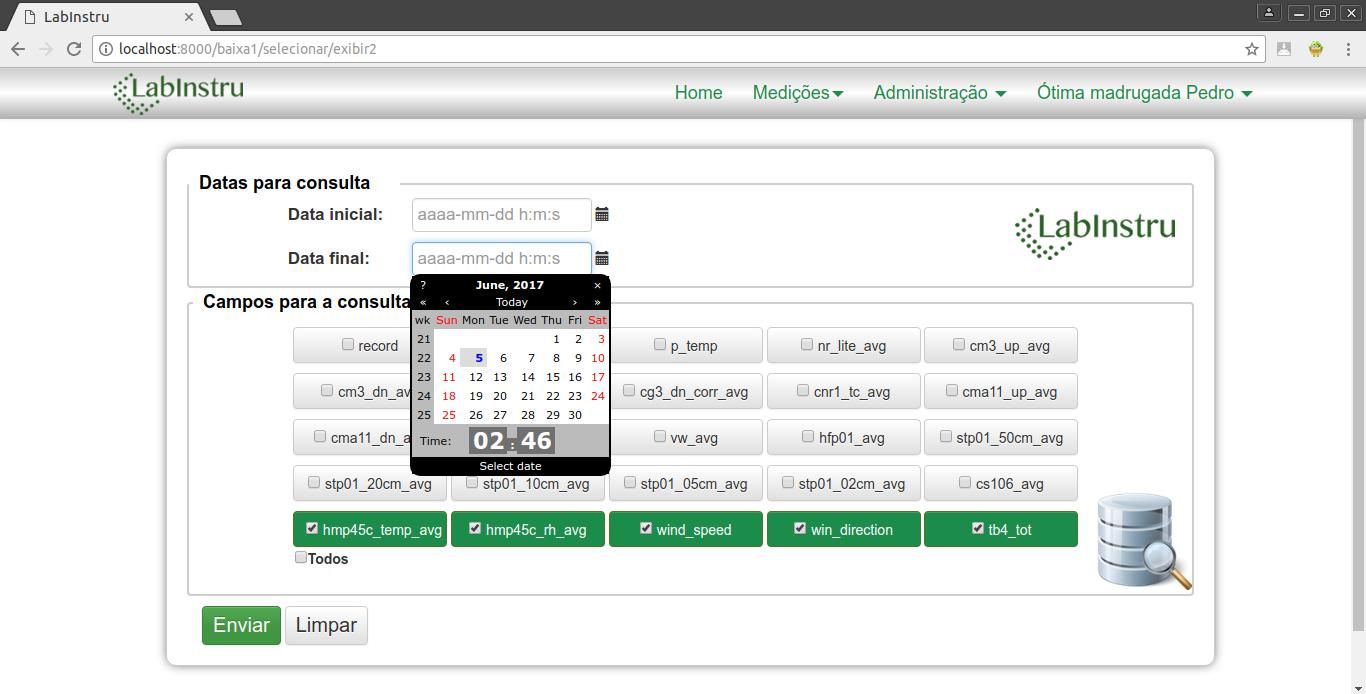
\includegraphics[width=0.7\linewidth]{./img/ap3}}
\caption{Consulta de medições.}
\end{figure}
\end{frame}

\begin{frame}{Solução Proposta: Funcionalidades Implementadas}
\begin{figure}[h!]
\centering
\frame{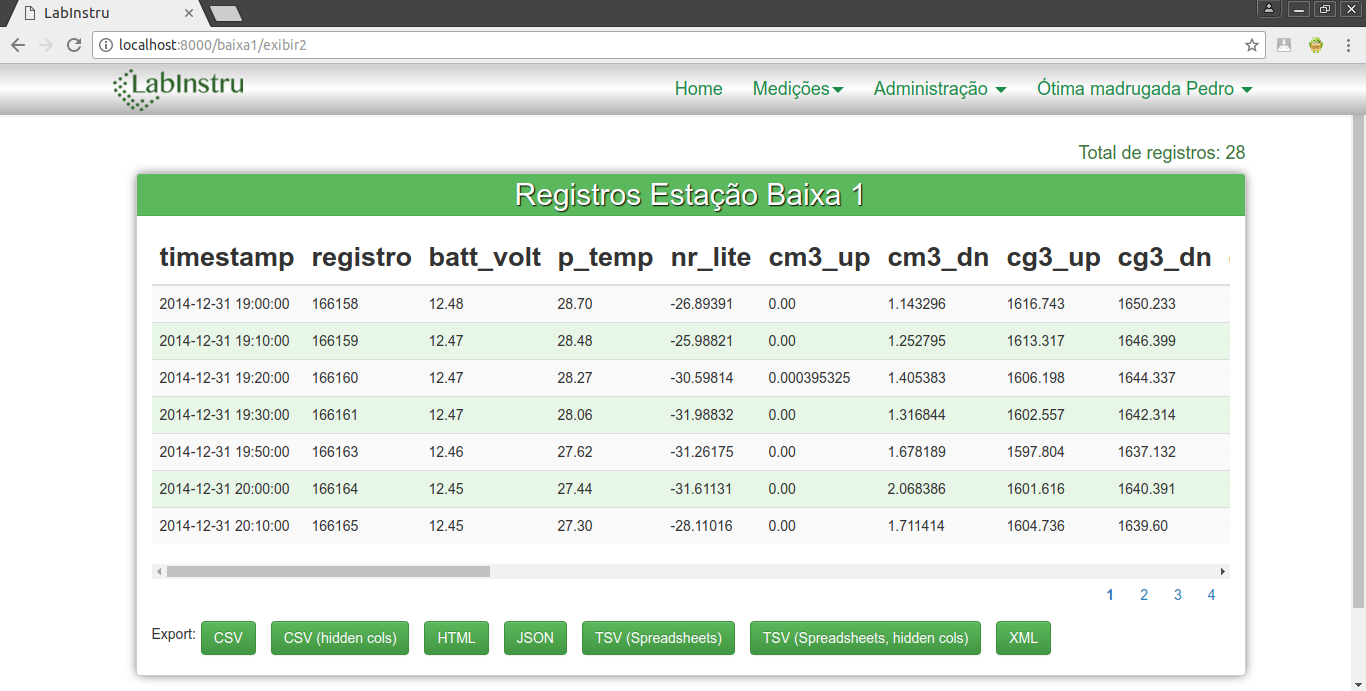
\includegraphics[width=0.7\linewidth]{./img/ap7}}
\caption{Resultado da consulta de medições.}
\end{figure}
\end{frame}

\begin{frame}{Solução Proposta: Funcionalidades Implementadas}
\begin{figure}[h!]
\centering
\frame{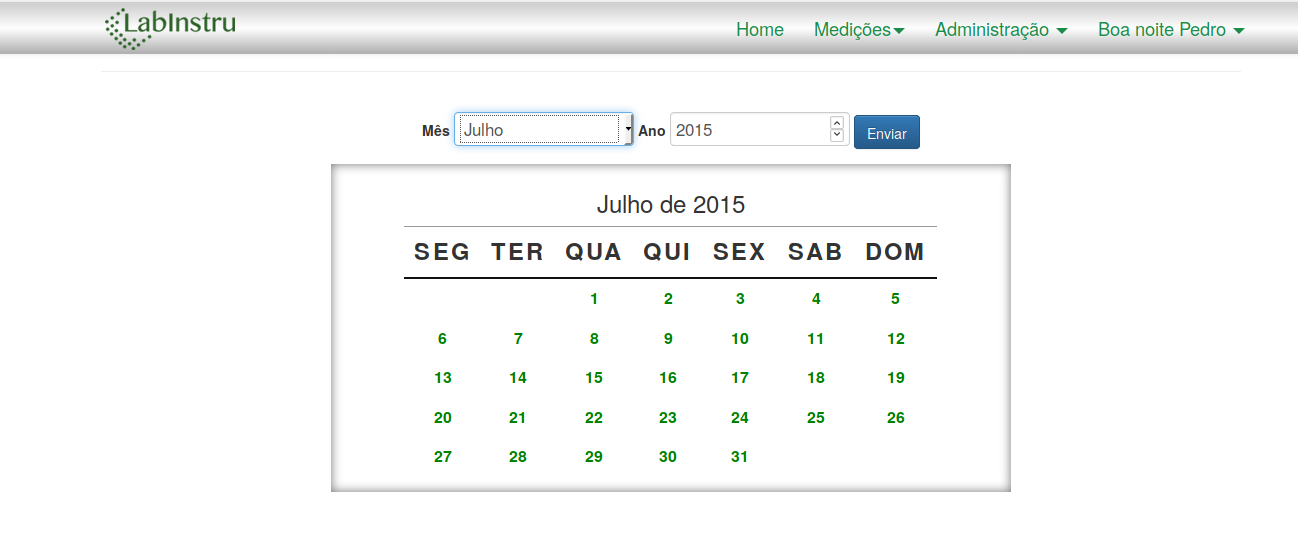
\includegraphics[width=0.7\linewidth]{./img/disponibilidade2}}
\caption{Verificação de disponibilidade}
\end{figure}
\end{frame}

\begin{frame}{Apresentação LabInstru Web}
	\begin{center}
	\movie[width=160px, height=90px, externalviewer]{Vídeo de ilustração de algumas funcionalidades.}{video/video.mp4}
	\end{center}
\end{frame}

\begin{frame}{Boletim Meteorológico Diário}
\begin{itemize}
	\item Uma das atividades promovidas pelo LabInstru
	\item Importante informativo sobre clima e tempo de nossa região
  \item Divulgação das informações junto à comunidade
	\item Possui várias informações derivadas dos dados obtidos da estação meteorológica
	\begin{itemize}
		\item Índice de Calor
		\item Escala de Beaufort
	\end{itemize}
	\item Elaboração de modelo para o boletim meteorlógico
	\item Implementação a partir do modelo
\end{itemize}
\end{frame}

\begin{frame}{Modelo para Boletim Meteorológico Diário}
\begin{figure}[h!]
\centering
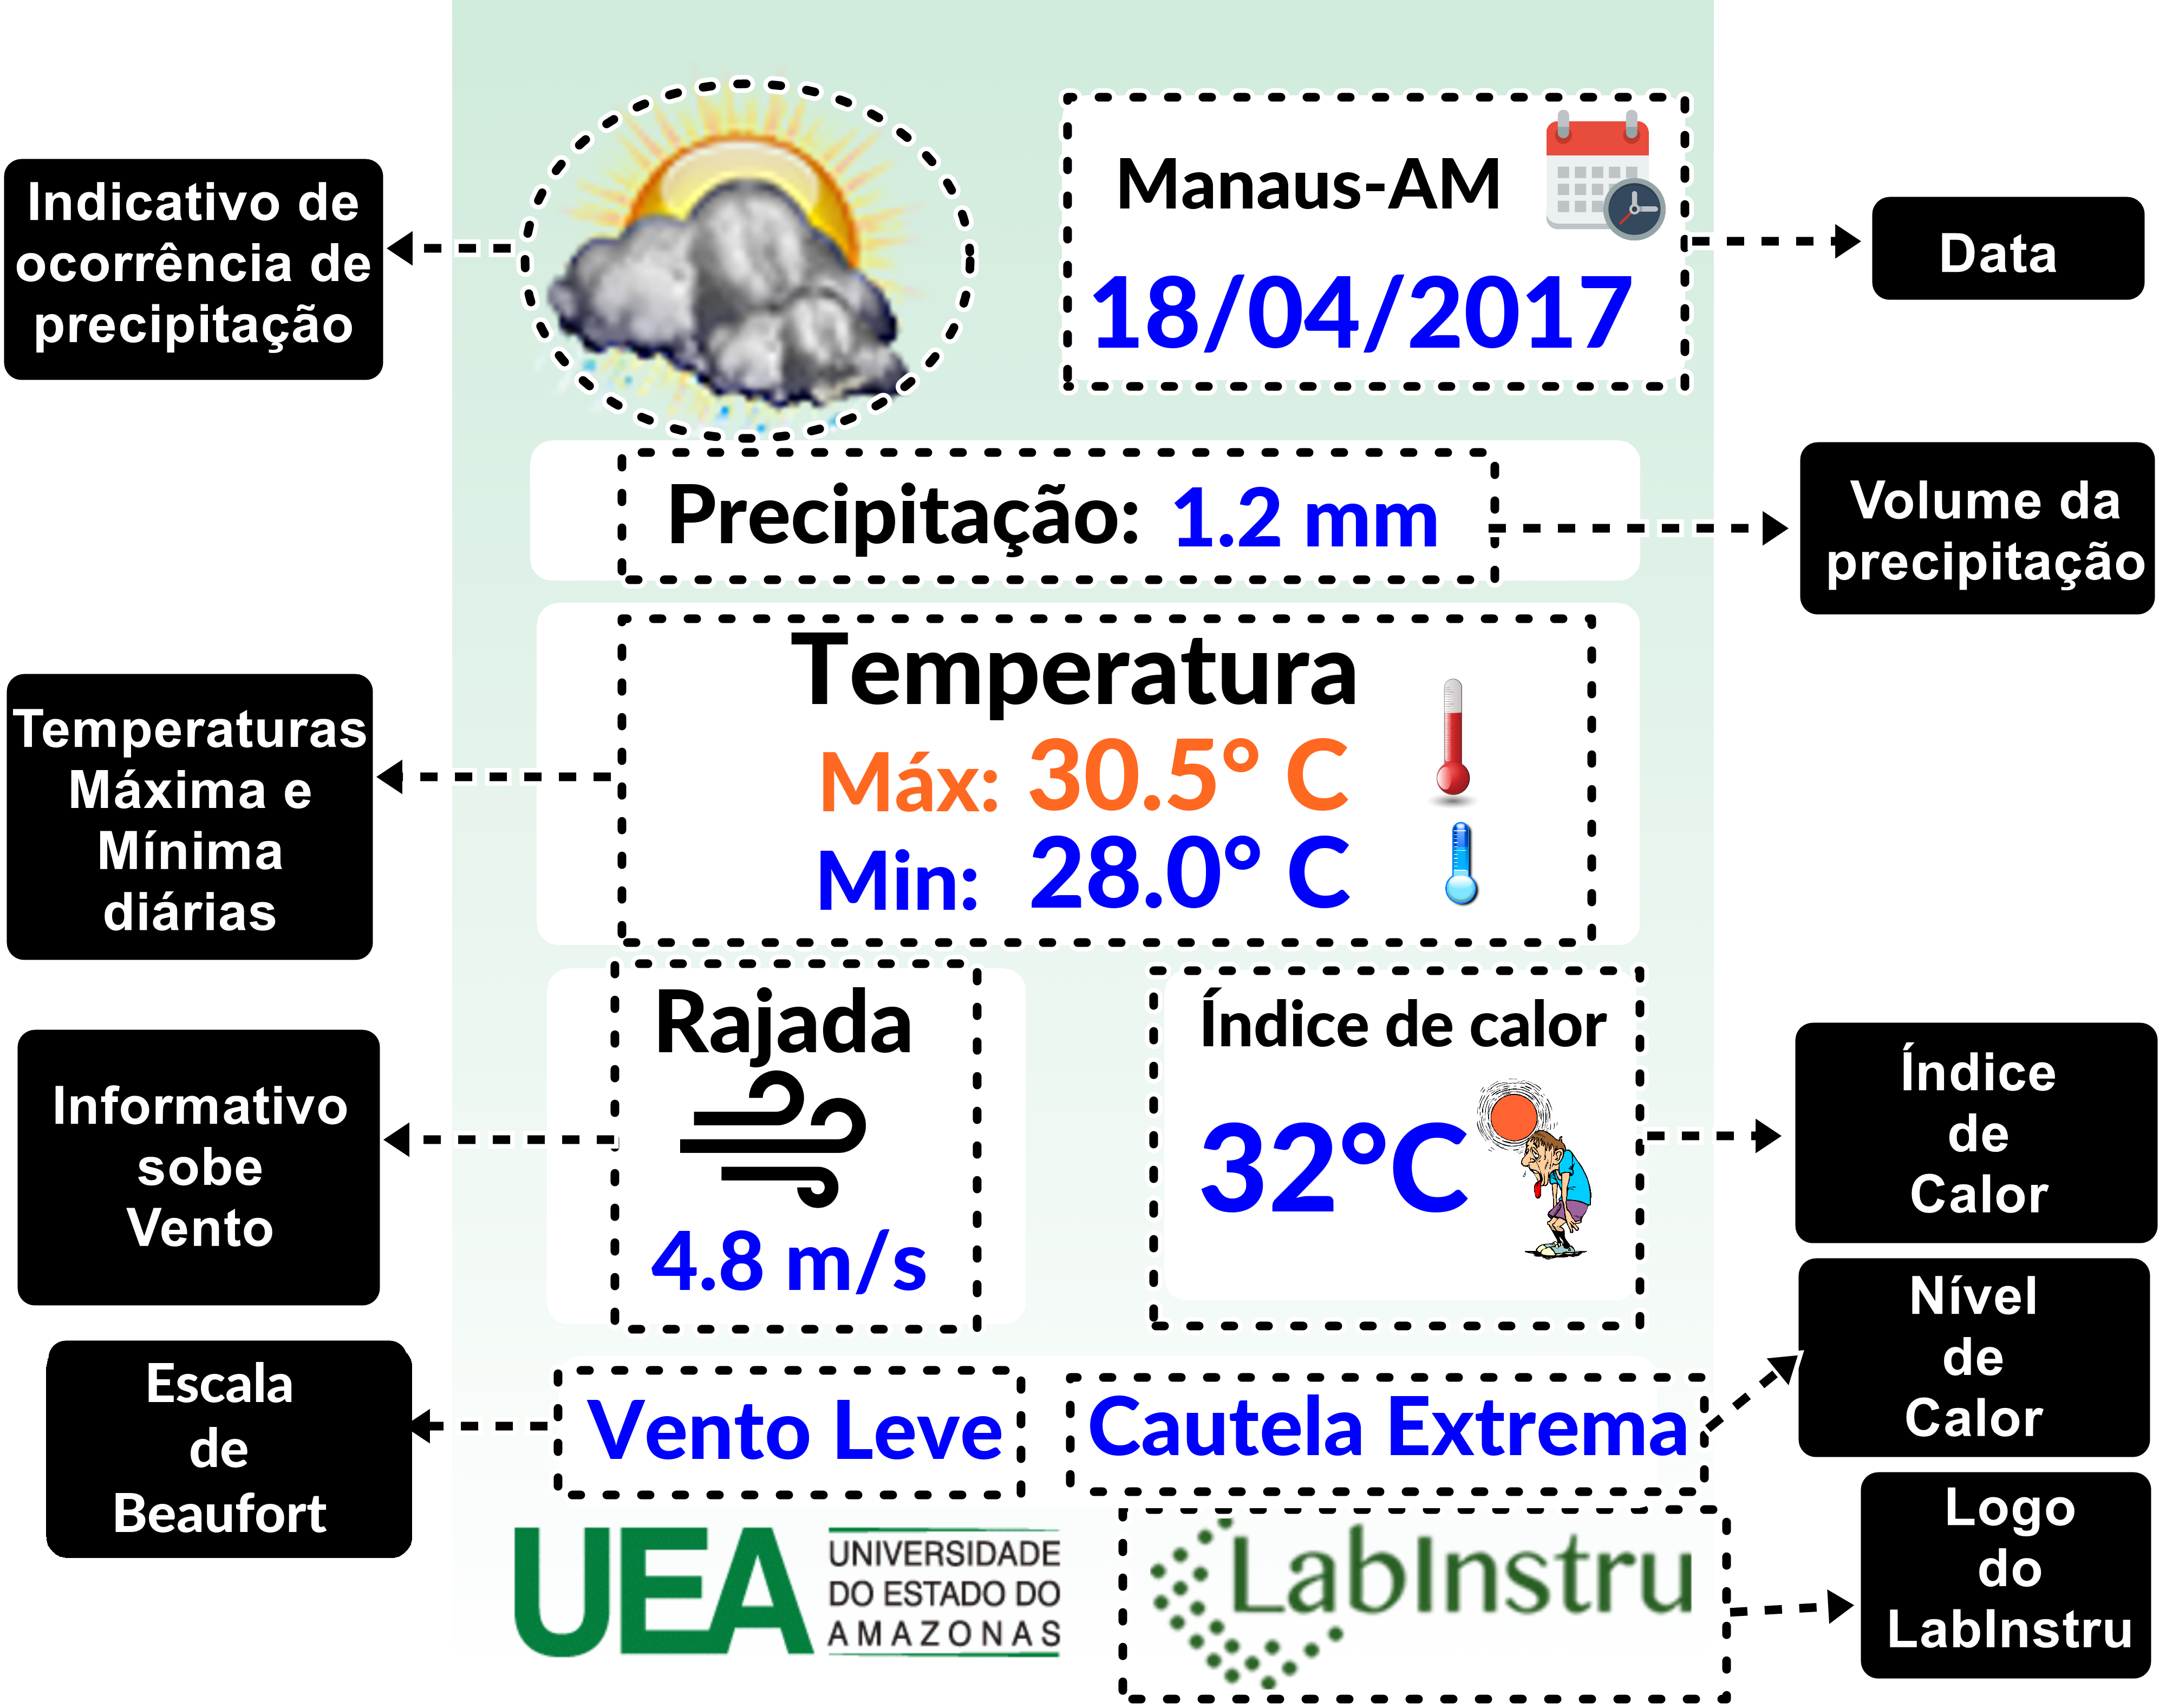
\includegraphics[width=0.5\linewidth]{./img/esbocoBoletim}
\caption{Modelo elaborado para o boletim meteorológico} \label{fig:modeloBoletim}
\end{figure}
\end{frame}

\begin{frame}{Boletim Meteorológico Diário Implementado}
\begin{figure}[h!]
\centering
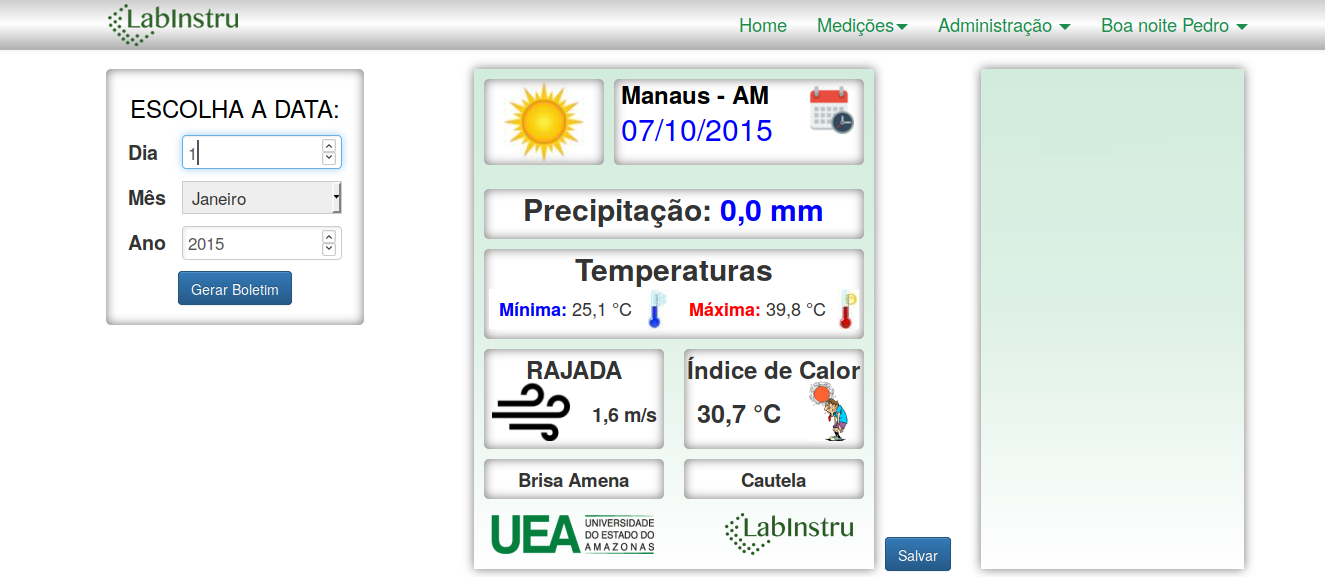
\includegraphics[width=0.7\linewidth]{./img/boletim}
\caption{Boletim meteorológico implementado no LabInstru Web} \label{fig:boletim}
\end{figure}
\end{frame}

\begin{frame}{Métricas de Software}
\begin{itemize}
\item Linhas de código: 7264 no total, sendo:
\begin{itemize}
\item[-] Arquivos Python: 1714 linhas
\item[-] Arquivos HTML: 2400 linhas
\item[-] Arquivos de estilo: 3150 linhas
\end{itemize}
\ \ \newline
\item Funções disponíveis no Controller: 28
\begin{itemize}
	\item Analogia com web services
\end{itemize}
\ \ \newline
\item Modelo de dados: 8
\begin{itemize}
	\item Acordância com a modelagem efetuada anteriormente
\end{itemize}
\end{itemize}
\end{frame}


\begin{frame}{Implantação da Solução Proposta}
\begin{itemize}
	\item Realizada com o \alert{Google App Engine}
	\begin{itemize}
		\item Plataforma em nuvem
		\item Total suporte à linguagem Python
		\item Nível de serviço gratuito
		\item Alta disponibilidade e baixa latência
	\end{itemize}
	\ \ \newline
	\item \alert{Status atual}: Corrigindo detalhes de implantação para disponibilização aos pesquisadores e estudantes do LabInstru
\end{itemize}
\end{frame}
